\documentclass[letterpaper,11pt]{article}

\usepackage{amsmath}
\usepackage{amssymb}
\usepackage{graphicx}
\usepackage{algorithm}
\usepackage{algorithmic}

\newcommand{\PM}{PYroMat}
\def\d{\mathrm{d}}

\title{The Thermodynamic Models in PYroMat}
\author{Christopher R. Martin}
\date{\today}

\begin{document}

\maketitle

\section*{Nomenclature}

\section{Introduction}

\section{Ideal Gases}

\subsection{Introduction}


\section{Multi-phase properties}

\section{Efficiently evaluating polynomials and their derivatives}

It must be clear from the previous sections that polynomials are an important tool for accurately modeling thermodynamic properties.  However, how they are best evaluated in code is more nuanced than it may seem.  

For example, if we were to evaluate $x^4$, we might use \verb|x**4| in Python or we might use \verb|x*x*x*x|.  Which is better?  The answer depends on how much data we are analyzing (recall that \PM\ supports arrays).

Figure \ref{fig:benchmark} shows the results of a computation time study on the time to multiply Numpy arrays of different sizes.  The \verb|**| and \verb|np.power| operations were shown to be equivalent.  Certainly on faster or slower processors, the time scale might be faster or slower, but the shape of the curve will probably be roughly the same.  Some machines with different array operation support may see slightly different relative performance curves, but these are probably quite characteristic for most machines.

\begin{figure}
\centering
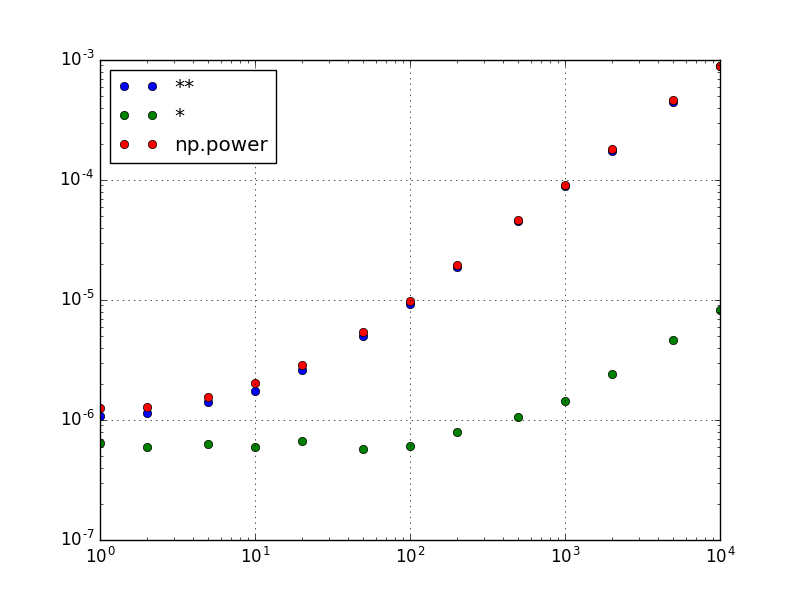
\includegraphics[width=.97\linewidth]{benchmark}
\caption{Computation time for array multiplication, and power operations.}\label{fig:benchmark}
\end{figure}

For small data sets (fewer than 10 or so elements), the overhead dominates the computational time, so adding array elements has little or no impact.  We could probably only perform two or three multiplications before the costs start to appear equal.  On the other hand, the computational costs are so small in these cases, it probably doesn't matter whether we use multiplication or exponents.

The real cost appears when data sets are larger.  By the time the arrays are over 1,000 elements, it is clear that multiplication and exponents diverge in their cost.  On a 10,000 element array, 100 multiplications can be performed for the cost of a single exponent and that trend only worsens with larger arrays.

The conclusion is that exponents should be used rarely (if ever) and repeated multiplications are dramatically more efficient.  This is somewhat less true on small data sets where there is significant computational overhead, but these operations are also so inexpensive to begin with, that there is little pressure on optimizing for those cases.

The remaining question is how best to minimize the number of multiplications.

\subsection{Polynomials of one variable}

Polynomials of one variable may be expressed
\begin{align}
p(x) = c_0 + c_1 x + c_2 x^2 + c_3 x^3 + \ldots
\end{align}
We have made the case that it is preferable to express $x^3$ as $x\times x\times x$, but if that is the case, $x \times x$ would already have been available when calculating $x^2$, so we should absolutely avoid redundant operations.  An $N^\mathrm{th}$ order polynomial would imply $N(N-1)$ multiplications and $N$ additions.  On the other hand, if the polynomial were to be evaluated as
\begin{align}
p(x) = c_0 + x(c_1 + x(c_2 + x(c_3 + \ldots
\end{align}
there are only $N$ multiplications and $N$ additions.

While numerically expedient, it leads to a very awkward notation.  Instead, consider the polynomial constructed from a series of intermediate polynomials, $p_k(x)$.  For an $N^\mathrm{th}$ order polynomial,
\begin{subequations}
\begin{align}
p_N(x) &= c_N\\
p_k(x) &= c_k + xp_{k+1}(x) \hspace{1em} \forall\ k\ :\ 0 \le k < N\\
p_0(x) &= p(x).
\end{align}
\end{subequations}
This formulation invites an approach for calculating the polynomial numerically, but it also suggests a convenient method for efficiently calculating the derivative of the polynomial.
\begin{subequations}
\begin{align}
p'_N(x) &= 0\\
p'_k(x) &= p_{k+1}(x) + xp'_{k+1}(x)\\
p'_0(x) &= p'(x)
\end{align}
\end{subequations}
This operation requires $N$ additional multiplications and $N$ additional additions.

The same approach may be extended to a second derivative,
\begin{subequations}
\begin{align}
p''_N(x) &= 0\\
p''_k(x) &= 2p'_{k+1}(x) + xp''_{k+1}(x)\\
p''_0(x) &= p''(x),
\end{align}
\end{subequations}
or to an arbitrary derivative, $(l)$,
\begin{subequations}
\begin{align}
p^{(l)}_N(x) &= 0\\
p^{(l)}_k(x) &= lp^{(l-1)}_{k+1}(x) + xp^{(l)}_{k+1}(x)\\
p^{(l)}_0(x) &= p^{(l)}(x).
\end{align}
\end{subequations}
Each derivative requires an additional $2N$ multiplications and $N$ additions for a total of $N(2l+1)$ multiplications and $Nl$ additions.

At this stage, the notation has grown to be somewhat difficult to parse.  It would appear that a two-dimensional array of intermediate values $N\times l$ is necessary.  However, careful examination of these expressions show that if they are evaluated in the correct order, the values of previous steps can be overwritten.  For clarity, we demonstrate in Algorithm \ref{alg:1d:poly} with only the second-order derivative.

\begin{algorithm}
\caption{The calculation of a polynomial of one variable and two derivatives}\label{alg:1d:poly}
\begin{algorithmic}
\REQUIRE A series of $N$ real coefficients, $c_k$
\REQUIRE A value, $x$
\STATE Declare results $p_0$, $p_1$, and $p_2$
\STATE Initialize:
\STATE $p \leftarrow c_N$
\STATE $p_x \leftarrow 0.0$
\STATE $p_{xx} \leftarrow 0.0$
\FOR{$k$ from $N-1$ to 0}
\STATE $p_{xx} \leftarrow 2p_1 + x p_2$
\STATE $p_x \leftarrow p_0 + x p_1$
\STATE $p \leftarrow c_k + x p_0$
\ENDFOR
\RETURN $p_0$, $p_1$, $p_2$
\end{algorithmic}
\end{algorithm}
It should be emphasized that the earliest values of the higher-order derivatives will always be zero.  It is possible to spare the operations spent constructing these elements, but it is dubious whether the added complexity will be worth it.  \PM\ only needs to calculate the second derivative (at most) of any polynomial, so there is little interest in sparing the additional two multiplications that implies.

\subsection{Polynomials with non-integer exponents}

With little loss of efficiency, it is possible to perform a pre- and post-transformation to allow the above algorithm to function with non-integer exponents.  Consider
\begin{align}
p(x) = x^b \hat{p}(x^a)
\end{align}
The pre-exponent, $a$, and post-exponent, $b$, need not be integers, and they need not be positive.  When $\hat{p}$ is a polynomial with strictly integer exponents, 
\begin{align}
p(x) = c_0 x^a + c_1 x^{a+b} + c_2 x^{2a+b} + c_3 x^{3a+b} + \ldots
\end{align}
The $k^\mathrm{th}$ term takes the form $c_k x^{ka+b}$.

So, for example, the polynomial,
\begin{align}
p(x) = 2 x^{0.2} + 3 x^{0.6} + x
\end{align}
might be alternately expressed as quadratic with a 0.4 pre-exponent and a 0.2 post-exponent,
\begin{align}
p(x) = x^{0.2} \left( 2 + 3 x^{0.4} + (x^{0.4})^2 \right)
\end{align}

Great care should be taken, though, since a single exponent can be as expensive as 100 multiplications for arrays of any size.  So, even with this support large exponents should not be reduced.  For example, the polynomial
\begin{align}
p(x) = 4x^{26} + 7x^{28},
\end{align}
can be conveniently expressed as linear with a pre-exponent of 2 and a post exponent of 26,
\begin{align}
p(x) = x^{26} \left( 4 + 7(x^2) \right).
\end{align}
Two exponents are far more expensive than 28 multiplications except on trivially small data sets, so this type of formulation should be avoided.

Derivatives with pre- and post-exponents are calculated in the usual way.  For example, the first derivative is
\begin{align}
p'(x) = bx^{b-1} \hat{p}(x^a) + a x^{b+a-1} \hat{p}'(x^a).
\end{align}
It should be more clear now than ever that these pre- and post-exponentials are powerful, but they carry a steep numerical cost.

\subsection{Polynomials of two variables}

The multi-phase class depends heavily on polynomials of two variables.  These can be expressed in the form
\begin{align}
p(x,y) = \sum_{i,j}^{N,M} c_{i,j} x^i y^j.
\end{align}
This might be written as
\begin{align}
\begin{array}{rccccl}
c_{0,0} & + & c_{0,1} y & + & c_{0,2} y^2 & +\ldots\\
x\big(c_{1,0} & + & c_{1,1} y & + & c_{1,2} y^2 & +\ldots \big)\\
x^2\big(c_{2,0} & + & c_{2,1} y & + & c_{2,2} y^2 & +\ldots \big)\\
+\ldots & & & & &
\end{array}
\end{align}
Clearly, there is the potential for economy of calculations to keep a running tab of multiples of $x$ and $y$ and apply each to the terms where they appear.  However, this approach requires arrays of intermediate values.  Worse still, when the additional multiplications required to apply the coefficients are considered, there is not really any gain in performance over a nested polynomial approach used previously on polynomials of one variable.

To this end, we define a polynomial on $y$, representing one of the rows above, all having the same power of $x$,
\begin{align}
q_i(y) = c_{i,0} + y ( c_{i,1} + y ( c_{i,2} + y ( \ldots
\end{align}
This is merely a polynomial on one variable, and it can be evaluated in precisely the same manner as above,
\begin{subequations}
\begin{align}
q_{i,M}(y) &= c_{i,M}\\
q_{i,j}(y) &= c_{i,j} + y\,q_{i,j+1}(y)\\
q_{i,0}(y) &= q_i(y).
\end{align}
\end{subequations}
Now, the polynomial on $x$ is constructed by the same approach, but its coefficients on $x$ are replaced by $q_i(y)$ instead.
\begin{subequations}
\begin{align}
p_N(x,y) &= q_{N,0}(y)\\
p_i(x,y) &= q_{i,0}(y) + x p_{i+1}(x,y)\\
p_0(x,y) &= p(x,y).
\end{align}
\end{subequations}

Evaluation of the partial derivatives of $p(x,y)$ can be carried out in using the same approach as was done in polynomials of one variable, but there is some additional complexity due to the nested evaluation scheme.  Consider the problem of calculating $\partial^{l+m} p / \partial x^l \partial y^m$.

Let us begin with derivatives on the inner polynomials, $q(y)$.  The $m^\mathrm{th}$ derivative is
\begin{subequations}
\begin{align}
q^{(m)}_{i,M}(y) &= 0\\
q^{(m)}_{i,j}(y) &= m q^{(m-1)}_{i,j+1}(y) + y\,q^{(m)}_{i,j+1}(y)\\
q^{(m)}_{i,0}(y) &= q^{(m)}_{i}(y)
\end{align}
\end{subequations}
When $l$ (the x derivative order) is zero,
\begin{align}
p^{(0,m)}_N(x,y) &= q^{(m)}_{N,0}(y)\\
p^{(0,m)}_i(x,y) &= q^{(m)}_{i}(y) + x p^{(0,m)}_{i+1}(x,y)\\
p^{(0,m)}_0(x,y) &= \frac{\partial^{m}}{\partial y^m}p(x,y),
\end{align}
and when $l$ is not zero,
\begin{align}
p^{(l,m)}_N(x,y) &= 0.\\
p^{(l,m)}_i(x,y) &= l p^{(l-1,m)}_{i+1}(x,y) + x p^{(l,m)}_{i+1}(x,y)\\
p^{(l,m)}_0(x,y) &= \frac{\partial^{l+m}}{\partial x^l \partial y^m}p(x,y).
\end{align}

Algorithm \ref{alg:2d:poly} demonstrates how this can be implemented 

\begin{algorithm}
\caption{A polynomial on two variables and with second derivatives.}\label{alg:2d:poly}
\begin{algorithmic}
\REQUIRE An ($N\times M$) array of coefficients: $c_{i,j}$
\STATE Initialize a $p$ and derivatives:
\STATE $p, p_x, p_y, p_{xx}, p_{xy}, p_{yy} \leftarrow 0$
\FOR{$i$ from $N$ to 0}
    \STATE Initialize $q$ and derivatives:
    \STATE $q \leftarrow c_{N,M}$
    \STATE $q_y \leftarrow 0.0$
    \STATE $q_{yy} \leftarrow 0.0$
    \FOR{$j$ from $M-1$ to 0}
        \STATE $q_{yy} \leftarrow 2 q_y + y q_{yy}$
        \STATE $q_y \leftarrow q + y q_y$
        \STATE $q \leftarrow c_{N,j} + y q$
    \ENDFOR
    \STATE $p_{xx} \leftarrow 2 p_x + x p_{xx}$
    \STATE $p_{xy} \leftarrow p_y + x p_{xy}$
    \STATE $p_{yy} \leftarrow q_yy + x $
    \STATE $p_x \leftarrow p + x p_x$
    \STATE $p_y \leftarrow q_y + x p_y$
    \STATE $p \leftarrow q + x p$
\ENDFOR
\RETURN $p$, $p_x$, $p_y$, $p_{xx}$, $p_{xy}$, $p_{yy}$
\end{algorithmic}
\end{algorithm}

The approach presuming a densely populated $M\times N$ array of coefficients is prudent so long as there are not many elements of $c_{i,j}$ that are zero.  When $c$ is very sparsely populated, a different approach is warranted.  

\PM\ uses a coordinate sparse approach to representing polynomials.  In this method, all coefficients in the $M \times N$ array are assumed to be zero unless they are explicitly listed with their values.  Each coefficient is specified along with its integer $x$- and $y$-exponent, which corresponds to its place in the array.

It is convenient for evaluating these polynomials if the coefficients can be listed in descending exponent order.  A nested loop can be constructed to iterate over $x$ and then $y$ exponents.  If the exponent is not found in the coefficient array, the coefficient is treated as zero.  

\begin{algorithm}
\caption{POLY2 evaluation of a polynomial of two variables}\label{alg:poly2}
\begin{algorithmic}
\REQUIRE Arrays $a_k,b_k,c_k$ with $D$ elements representing $D$ nonzero terms\\
For the $k^\mathrm{th}$ term:\\
$a_k$ is the power of $x$\\
$b_k$ are the powers of $y$\\
$c_k$ is the coefficient
\REQUIRE The coefficient order is sorted in descending order of $a_k$
\REQUIRE Terms with the same values of $a_k$\\
are sorted in descending order of $b_k$.\\
\STATE $p, p_x, p_y, p_{xx}, p_{xy}, p_{yy} \leftarrow 0$\\
$M$ and $N$ are be the $x$ and $y$ polynomial orders
\STATE $M \leftarrow a_0$
\STATE $k \leftarrow 0$
\STATE \COMMENT{This loop iterates over $x$ exponents}
\FOR{$i$ from $M$ to $0$}
    \STATE $q,q_y,q_{yy} \leftarrow 0$
    \STATE \COMMENT{If $i$ matches the next nonzero $x$-exponent}
    \IF{$k < D$ \AND $a_k$ is $i$}
        \STATE $N \leftarrow b_k$
        \FOR{$j$ from $N$ to $0$}
            \STATE $q_{yy} \leftarrow 2 q_y + y q_{yy}$
            \STATE $q_y \leftarrow q + y q_y$
            \STATE \COMMENT{If $i$ and $j$ match the next nonzero $x$- and $y$-exponents}
            \IF{$k<D$ \AND $a_k$ is $i$ \AND $b_k$ is $j$}
                \STATE $q \leftarrow c_k + y q$
                \STATE $k \leftarrow k+1$
            \ELSE
                \STATE $q \leftarrow y q$
            \ENDIF
        \ENDFOR
    \ENDIF
    \STATE $p_{yy} \leftarrow q_{yy} + x p_{yy}$
    \STATE $p_{xx} \leftarrow 2 p_x + x p_{xx}$
    \STATE $p_{xy} \leftarrow p_y + x p_{xy}$
    \STATE $p_x \leftarrow p + x p_x$
    \STATE $p_y \leftarrow q_y + x p_y$
    \STATE $p \leftarrow q + x p$
\ENDFOR
\end{algorithmic}
\end{algorithm}


\subsection{Implementation of the algorithm}
In practice, this cumbersome notation can be drastically simplified in code because it is not necessary to distinguish between $p$ and $q$ in their various iterations; provided care is taken not to overwrite a value before it is needed.

In most practical polynomials of two variables of given order, very few of the possible coefficients may be non-zero, so storing and looping over all $m\times n$ coefficients may not be sensible.  Instead, it is common to take an approach closer to spare matrix storage.

If we have one-dimensional arrays of polynomial coefficients, $c_k$, and exponents, $a_k$ and $b_k$, the polynomial will be constructed as
\begin{align}
p(X,Y) = \sum_k=0^{N-1} c_k X^{a_k} Y^{b_k}.
\end{align}
In this way, the polynomial
\begin{align}
p(X,Y) = -0.1 X^2 + XY + 0.5 Y^2 - Y - 0.2
\end{align}
may be represented by
\begin{align}
a &= \left[ 2,\ 1,\ 0,\ 0,\ 0\right]\\
b &= \left[ 0,\ 1,\ 2,\ 1,\ 0\right]\\
c &= \left[ -0.1,\ 1,\ 0.5,\ -1,\ 0.2\right]
\end{align}

For the algorithm to function efficiently, it is reasonable to impose some prior sorting of the exponent values.  Since the series above requires that we interact with higher-order terms first, let us assert that the polynomial should be expressed in order of descending exponents on $X$ and then $Y$.

In Algorithm \ref{alg:poly2}, we employ an outer loop on the values of $i$ and an inner loop on the values of $j$.  If coefficients are absent from the arrays (if the $i,j$ pair is not found), then the coefficient is presumed to be zero.  Starting with the maximum value for each exponent, the indices are reduced incrementally until the $i,j$ combination corresponding to the next row ($k$) is found.

This is extremely practical for polynomials where most of the possible combinations are not represented, and does not cost much for cases where they are.

\end{document}
